\documentclass[12pt]{article}
\usepackage{fullpage, graphicx, url}
\setlength{\parskip}{1ex}
\setlength{\parindent}{0ex}
\title{PUMA 3.1 Guided Tour}
\begin{document}

\section*{Welcome to PUMA 3.1!}
\addcontentsline{toc}{section}{Welcome to PUMA 3.1!}

\tableofcontents

\subsection*{Introduction}
\addcontentsline{toc}{subsection}{Introduction}

PUMA 3.1 is a combination wiki and content management system. By now, you've installed the database and your site/ directory, and are ready to begin creating content. This document will take you on a guided tour through PUMA, including page creation, editing, and uploading files.

To begin, load up the main index page.

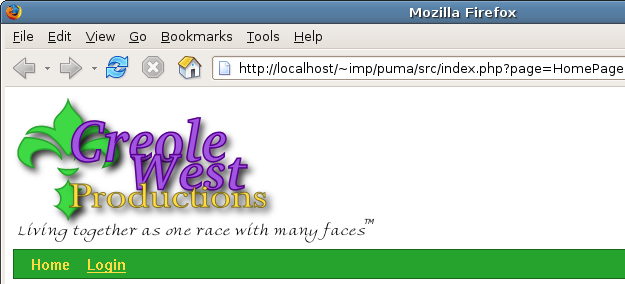
\includegraphics[scale=0.75]{images/tour1.png}

As you can see, the base site design I'm using is for Creole West Productions, who have generously sponsored development of PUMA. Your home page will look different, of course.

\subsection*{Logging In}
\addcontentsline{toc}{subsection}{Logging In}

Right now, we can't do anything, not even edit the main page! This is because we haven't logged in yet. Let's do that now.

During installation, you (or whoever installed PUMA for you) should have created a linkbar with links to important pages, like the HomePage and the UserPage.  We want to log in, so click on `Login' on the linkbar. 
\includegraphics[scale=0.75]{images/tour1a.png} The default installation has a user, admin, and the password is `password'. Go ahead and log in now.

If you don't have anything in the linkbar, then you'll need to modify it yourself.  See the `Advanced' section below.

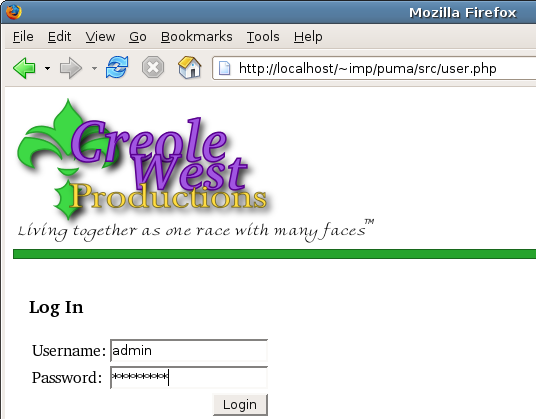
\includegraphics[scale=0.75]{images/tour2.png} 

Once you have logged in, you'll be taken to your user preferences page. Go ahead and return to the HomePage.

You'll notice that we now have some new options on the right side of the page.
 
 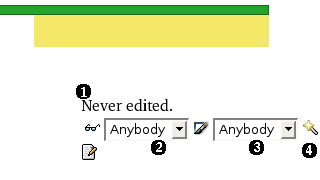
\includegraphics[scale=0.75]{images/tour3.png} 

First, we're told when the page was last edited (1). Below that, we have two access settings. PUMA has four different access levels: Anybody, Users, Editors and Admin. The first dropbox (2), to the right of the spectacles, determines who can view the page, while the second detemines who can edit the page (3). Note that, although you can set the page to be editable by Anyone, only users who are logged in may actually edit it. To the right of that is a wand (4), which allows us to set the permissions.

NOTE: You cannot set permissions the first time you edit a page!

\subsection*{Editing a Page}
\addcontentsline{toc}{subsection}{Editing a Page}

Let's create a HomePage. The final button is the `Edit Page' button. Click it now.

This will bring up the PUMA Editor, which acts just like a regular text editor with some PUMA-specific additions. For now, type in some sample text, and click `Preview Changes', which will show how the text will look on the page. Since this is just an example, go ahead and click `Save Changes'.

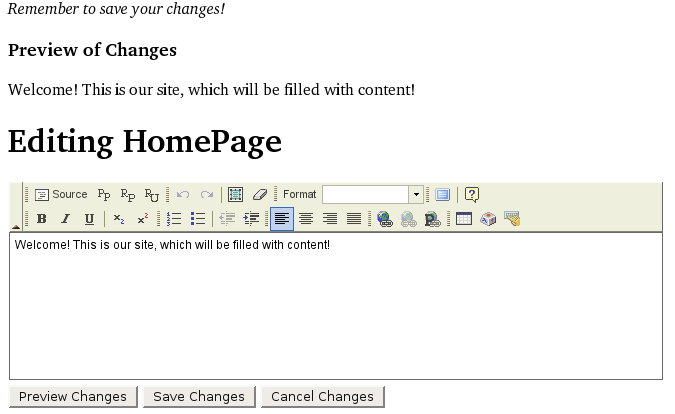
\includegraphics[scale=0.75]{images/tour4.png} 

If you had made some changes, but decided that you didn't like them after all, you could click `Cancel Changes' to leave the editor and return to the page you were editing.

We now have some more options on the right side of the page. We can see when the page was last edited, by whom, and which revision this is. We can also view the history of the page, by clicking on the book (1), or which pages link to the current page (2). We'll come back to these in a minute.

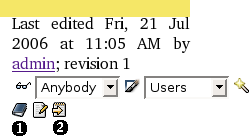
\includegraphics[scale=0.75]{images/tour5.png} 

\subsection*{The PagePicker and PUMA Plugins}
\addcontentsline{toc}{subsection}{The PagePicker and PUMA Plugins}

Now, lets take a look at some of the extra features in the editor.  In addition to having what you would expect to find--italics, bold, left justification, etc.--PUMA's editor has built-in functions to help you add resources, such as pictures; find pages and insert links to them; add links to PUMA's forums; and special links and values, such as the current date and reservations.

First, let's try out the PagePicker.

Click on the `PagePicker' link. 
\includegraphics[scale=0.75]{images/tour6.png}  By searching the titles and content of all pages in your site, the PagePicker can locate pages that currently exist and automatically insert the correct link for you. For example, type `home' in the search window, which will bring up suggested pages. Note that in this example, we only have the HomePage, so the PagePicker offers us only two choices: we can create a link to a new page called `home' or create a link to the HomePage.

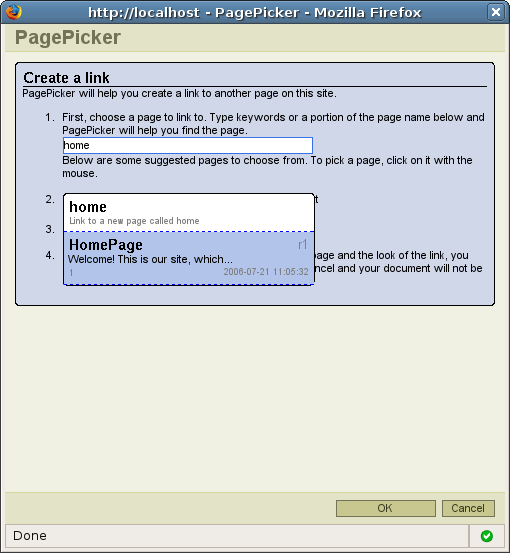
\includegraphics[scale=0.75]{images/tour7.png} 

Click on `HomePage', which will automatically fill in the rest of the options for you. We can change what the link text will look like in the next box. Let's change it to just `Home'. You'll see the preview automatically update below. We can now click on `OK' to insert the link, or cancel to exit out. Click OK.

Now, press space, and then click on the `PumaPlugin' link. 
\includegraphics[scale=0.75]{images/tour8.png}  This brings up the PumaPlugin dialog, with a list of all the available Puma Plugins. Let's add a link that will allow users to login and out, so select `User Login Link' and click OK.

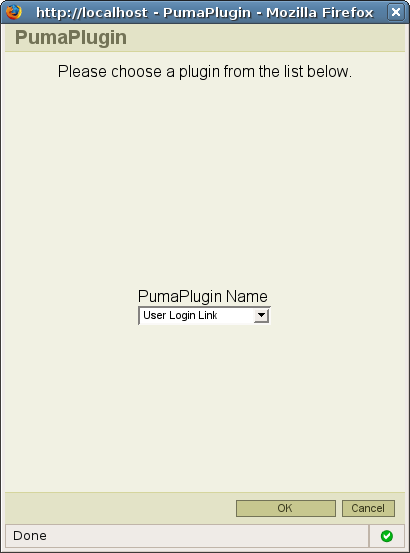
\includegraphics[scale=0.75]{images/tour9.png} 

The editor will show a graphic where the link will go, but a quick `Preview Changes' will show how it's replaced with, in our case, `admin'. This will change depending on the user, or, if no user is logged in, it will say, `Login'.

Let's see how to create a new page. This will be the ever-important `Contact Information' page. Click on the PagePicker button again, and this time type `Contact' in the first box. You can see that the PagePicker can't find any relevant pages, so it offers to create a link to a new page. Go ahead and click on `Contact'. Everything else looks OK, so click `OK' to insert the link, and then save the page.

\subsection*{Creating a New Page}
\addcontentsline{toc}{subsection}{Creating a New Page}

Creating a new page is as easy as editing it, literally. Click the `Contact' link and then edit the page. Put in some contact information.

The editor also has a built-in character map and international keyboard. 
\includegraphics[scale=0.75]{images/tour11.png}  They function fairly standardly, and will not be discussed further here.

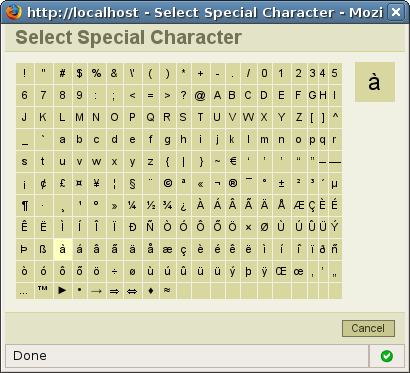
\includegraphics[scale=0.75]{images/tour11a.png} 

As a warning, some functions cannot be performed on the first edit of a page, (for example, the ResourcePicker and ResourceUploader, demonstrated below) because the page doesn't technically exist yet!

Save the contact page, and then return to the HomePage. Edit it.

\subsection*{Resources}
\addcontentsline{toc}{subsection}{Resources}

Suppose that we wanted to add a picture to the home page (or any other page, for that matter). How could we do that? We use the ResourceUploader and the ResourcePicker. 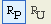
\includegraphics[scale=0.75]{images/tour12.png}  Click on the ResourceUploader first.

The `Nickname' is a short name to describe the resource--which can be nearly any type of file, not just an image--that you are uploading. Multiple files can have the same nickname; it is solely for your use. The `Description' is for a better description. You can click browse to pick out your file on the disk. When you're ready, click `Upload' to upload the file. If the upload is successful, you will get a message saying so.

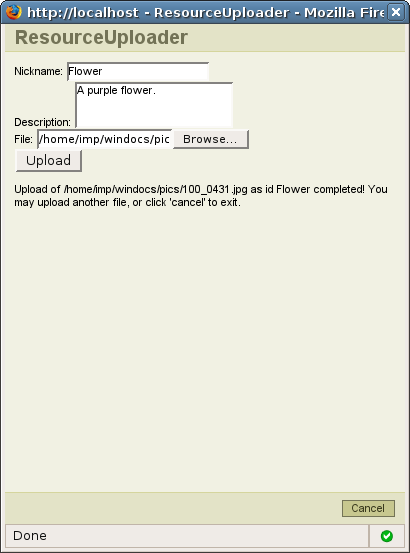
\includegraphics[scale=0.75]{images/tour13.png} 

You can upload more files or click `Cancel' to return to the editor.

Let's insert the image we just uploaded. Click on the ResourcePicker. The Resource Picker will find all resources associated with a particular page so you can attach them to the page. Images are displayed in the page itself; others are linked.

You can select the resource you want from the dropdown.

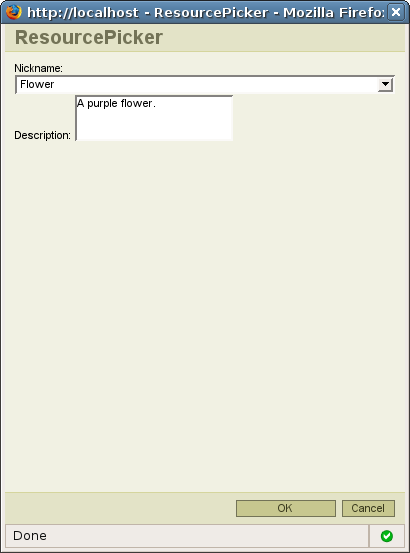
\includegraphics[scale=0.75]{images/tour14.png} 

The description will automatically change based on which resource you have chosen. Select the desired resource, and click OK. The ResourcePicker inserts the appropriate code into the editor.

Go ahead and save the changes to see the result. As you can see, the image has been inserted.

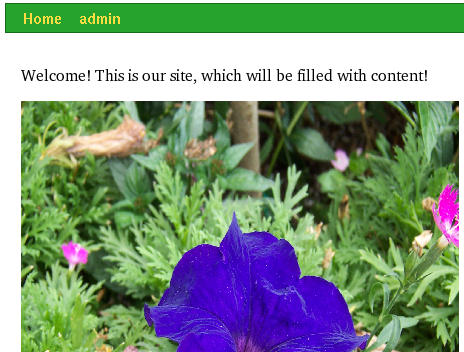
\includegraphics[scale=0.75]{images/tour15.png}

\subsection*{Examining Revisions}
\addcontentsline{toc}{subsection}{Examining Revisions}

Now, we can see the difference between two versions of a page by clicking on the `Compare to last' button on the right (1). 
\includegraphics[scale=0.75]{images/tour16.png}  This will give a detailed report of the most recent changes. (see below) We can also click on the `History' button (2) to see a list of all revisions, and go back to any previous version.

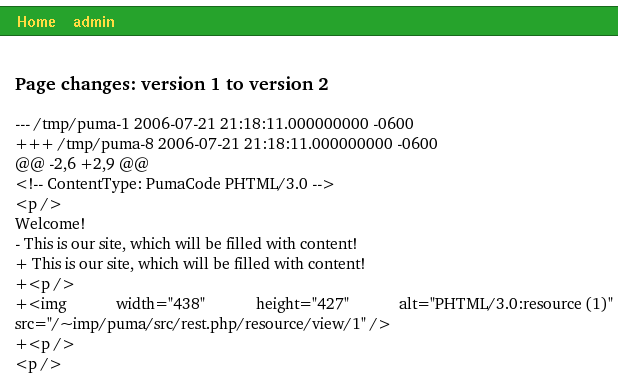
\includegraphics[scale=0.75]{images/tour17.png} 

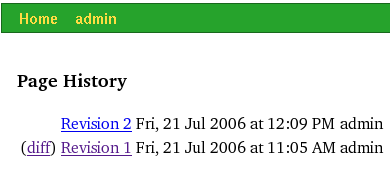
\includegraphics[scale=0.75]{images/tour18.png} 

 Finally, we should log out of PUMA for security. Click on the `admin' link in the linkbar to go to the user page. From there, click log out.

\section*{Advanced and Troubleshooting}
\addcontentsline{toc}{section}{Advanced and Troubleshooting}

\subsection*{Logging in when the Linkbar is Empty}
\addcontentsline{toc}{subsection}{Logging in when the Linkbar is Empty}

Change index.php to user.php in the browser's address bar, which will bring up the login page. PUMA, if you used the default SQL schema, comes with a default user, admin. The password is `password'.

\subsection*{Editing the Linkbar}
\addcontentsline{toc}{subsection}{Editing the Linkbar}

Replace `index.php' (and everything that follows it) with `edit.php?page=HeaderLink'. This will bring up the edit page for the link bar. Use the PagePicker for links to user-created pages in the site, and PumaPlugins for links to the user page.
\end{document}
